\documentclass[journal=jprobs,manuscript=article]{achemso}

\usepackage[version=3]{mhchem} % Formula subscripts using \ce{}
\usepackage[T1]{fontenc}       % Use modern font encodings
\usepackage{multirow}
\usepackage{subcaption}
\usepackage{booktabs}
\usepackage{hyperref}

\newcommand*\mycommand[1]{\texttt{\emph{#1}}}

\author{Stefan K. Solntsev}
\email{solntsev@wisc.edu}
\author{Michael R. Shortreed}
\author{Brian L. Frey}
\author{Lloyd M. Smith}
\affiliation[UwMadison]
{University of Wisconsin-Madison}
	
\title[Rapid and Accurate Global PTM Discovery (G-PTM-D) Using Post-Acquisition Spectral Calibration and Multi-Notch Searches]
  {Rapid and Accurate Global PTM Discovery (G-PTM-D) Using Post-Acquisition Spectral Calibration and Multi-Notch Searches}

\begin{document}

\begin{abstract}

Correct identification of protein post-translational modifications (PTMs) is crucial to understanding many aspects of protein function in biological processes.
G-PTM-D\citep{Li_2016} is a recently developed tool for global identification and localization of PTMs.
Spectral file calibration prior to applying G-PTM-D, and algorithmic enhancements in the peptide database search shown here significantly increase the accuracy and speed of PTM identification.
We enhance G-PTM-D by using targeted multi-notch searches, and demonstrate its effectiveness in identification of numerous types of PTMs, including high-mass modifications such as glycosylations.
The changes described in this work lead to a 20\% increase in the number of identified modifications and an order of magnitude decrease in the search time.
Targeted multi-notch searches are also shown to be useful in contexts other than G-PTM-D, producing superior results when used instead of standard narrow-window and open database searches.
\end{abstract}

\section{Introduction}

Many types of protein post-translational modifications (PTMs) are known, and databases containing detailed information about such modifications are readily available\citep{Creasy_2004}.
Information about a modification often includes the chemical or isotopic composition, mass, specificity to certain residues, and possible restriction of placement to peptide or protein termini.
Protein databases such as UniProt\citep{Uniprot_2017} include information on the localization of specific modifications to specific residues in the protein, but this information is far from complete.
Despite the extensive cataloging of the different protein modifications, their comprehensive discovery and identification in complex biological samples has continued to pose a challenge for proteomics\citep{Olsen_2013}.

Numerous procedures for identification and localization of PTMs from "bottom-up" tandem mass spectrometric datasets exist.
These primarily address common modifications (e.g. phosphorylations) in well-studied systems, but global discovery tools, such as MODa\citep{Na_2011} and G-PTM-D\citep{Li_2016}, for identification and localization of a wide variety of different PTMs are also available.
The G-PTM-D workflow consists of three stages: 1) A wide precursor mass tolerance database search ('open' search)\citep{Chick_2015, Na_2011}, which provides mass differences between the identified peptides and the observed precursor peptide masses (hypothesized to differ in mass due to the presence of a PTM);
2) For those peptides for which the mass difference corresponds to the mass of a known PTM, a database augmentation step adds plausible localized PTMs to the corresponding protein entries in the search database;
3) A final standard tight precursor tolerance search ('narrow-window' search) using the augmented database to identify both modified and unmodified peptides subject to the standard FDR threshold (e.g. 1\% FDR).

While G-PTM-D delivers confident identification of numerous types of PTMs, it has a few significant limitations.
The initial open search is slow, taking hours for modest size datasets.
Thus, high mass modifications such as glycosylations are out of reach, since widening the search window from the suggested $\pm 200$ Da increases the already-slow search time.
The final narrow-window search is also problematic, as it does not account for peptide-spectral matches (PSMs) with mass differences arising from misassignment of the monoisotopic peak during precursor deisotoping.
Discovery of modifications is limited to PTMs in the UniProt database: this is a significant limitation since that database does not include modifications arising from sample handling, and ignoring those modifications significantly degrades the final PTM identification rates.
Finally, PTMs that are similar in mass, such as phosphorylation (79.966331 Da) and sulfonation (79.956815 Da), are problematic since they are virtually indistinguishable in unprocessed spectral files.
These limitations motivated the work described here.

Spectral calibration is essential for distinguishing modifications with similar mass, and so we recommend running the G-PTM-D procedure on calibrated spectra files.
To address the long search times of the open search, we replace the search in the first stage by a specialized search called a multi-notch search that only allows specific mass differences which correspond to pre-selected masses (e.g. PTMs and amino acids).
This change improves the specificity of the search and significantly decreases search time.
The final narrow-window search is also replaced by a limited multi-notch search that accommodates errors in the precursor mass deisotoping (+1.0029 and + 2.0054), further increasing the number of confidently identified peptides and PTMs.
Finally, we replace the limited UniProt PTM list with a custom expanded list of modifications that includes chemical adducts, glycosylations, lipids, and other important modifications.
This change not only expands the list of identified and localized modifications, but also increases the number of confidently identified PSMs.
The enhanced G-PTM-D workflow is presented in Figure~\ref{fgr:diagram}.

\begin{figure}[H]
  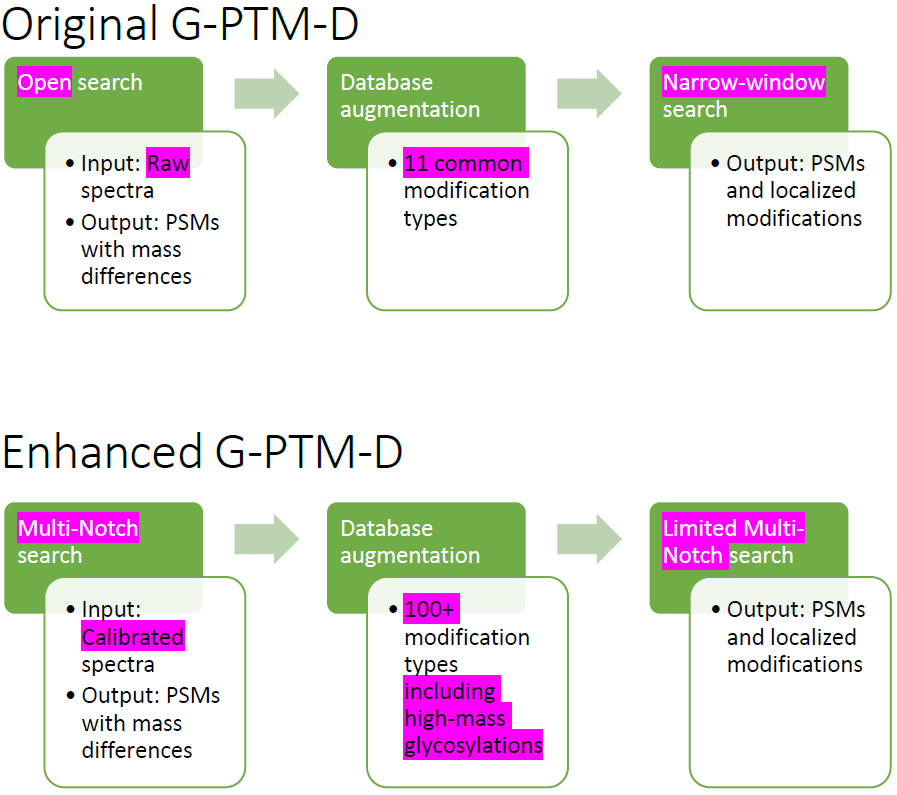
\includegraphics[scale=0.1]{paperDiagram.png}
  \caption{The three steps of the G-PTM-D workflow are indicated in the light beige color.}
  \label{fgr:diagram}
\end{figure}


\section{Experimental Procedures}

We developed a modified version of the Morpheus software for bottom-up spectral database searching\citep{Wenger_2013} that we call MetaMorpheus, which integrates the database search procedure with spectral calibration and the enhanced G-PTM-D workflow.
MetaMorpheus is freely accessible at \url{https://github.com/smith-chem-wisc/MetaMorpheus} as a standalone Windows executable program.
.NET Core versions, as well as the complete source code are available.
MetaMorpheus heavily utilizes an auxiliary library called mzLib, which is a vast library of software tools for analyzing and processing mass spectral data.
mzLib can be found at \url{https://github.com/smith-chem-wisc/mzLib}.

Three multi-fraction mammalian datasets with deep proteome coverage were used to evaluate performance.
These tryptically digested cell lysates correspond to 28 fractions from human Jurkat cells and 9 fractions from each of two different pancreatic islets from two species of mice.
These datasets are available at \url{https://db.systemsbiology.net/sbeams/cgi/PeptideAtlas/PASS_View?identifier=PASS00215} and \url{https://db.systemsbiology.net/sbeams/cgi/PeptideAtlas/PASS_View?identifier=PASS00470}, and are described in detail in~\citep{Shortreed_2015, Cesnik_2016}.

UniProt XML protein databases used were downloaded on Sept 14, 2017, and contain only reviewed human/mouse/contaminant proteins.

209 modifications including PTMs, adducts, and chemical modifications were allowed in the database augmentation step, see Supplementary Table 1 for a complete listing.

\section{Results and Discussion}

This work presents four major changes to the previously published G-PTM-D workflow:
a spectral calibration;
a replacement of the open search with a custom multi-notch search for PTM discovery;
replacement of the final traditional narrow mass search with a limited multi-notch search that permits exact matches even when incorrectly deisotoped precursor masses are present;
and lastly, addition of capacity for identification of multiple co-fragmented peptides from a single MS/MS scan.
To clarify the advantage of each change, they are first discussed separately, followed by an analysis of their combined effect upon overall G-PTM-D performance.

\subsection{Calibration}

A critical parameter for peptide identification is mass accuracy\citep{Scherl_2008}.
Higher mass accuracy provides increased specificity and thus confidence in peptide identifications, decreasing the false discovery rate.
Instrument noise, systematic drift and miscalibration all limit the mass accuracy in acquired spectra.
Multiple calibration strategies to improve mass accuracy have been devised and fall into three general categories: external calibration prior to the MS experiment (e.g. standard instrument calibration protocols); internal calibration during the MS experiment (e.g. real-time calibration using a lock mass standard\citep{Olsen_2005}); and spectral calibration subsequent to the MS experiment (post-acquisition spectral calibration).
We developed a post-acquisition calibration procedure that builds upon the software lock mass concept\citep{Cox_2011} recently reported by the Mann group.
In our strategy, the m/z differences between expected and observed peaks in the peptide tandem MS spectra are compiled, and then used to recalibrate the spectra.
The spectral calibration procedure consists of two steps: Step 1: A narrow tolerance (e.g. 10 ppm precursor, 0.01 Dalton fragment) database search is performed on the dataset.
This yields a set of peptide identifications subject to a desired false discovery rate (e.g. 1\% based upon the target:decoy strategy\citep{Elias_2007}).
Step 2: The identifications from Step 1 are used to extract peak matches from the spectra, and a peak shifting procedure is performed.
The calibration algorithm is described in detail in Supplementary Material 2.

We demonstrate the effectiveness of the calibration approach using a single CAST Mouse raw file as an example.
Figure~\ref{fgr:fig1-calibErrors} displays the errors in m/z values of MS1 peaks identified by Step 1 of the calibration, both before and after the calibration procedure is applied.
These errors are plotted versus two important variables: the m/z value of the peak and the retention time of the corresponding scan.
Calibration successfully removes both linear and non-linear dependencies between the m/z errors and these variables.
We note that in addition to these two parameters, the calibration function native to MetaMorpheus also considers peak intensity, injection time, total ion count, and other variables as potentially influencing the m/z errors.
MetaMorpheus calibrates both MS1 and MS2 scans (using MS2 fragment matches), but only the results from MS1 are shown here.
MetaMorpheus calibrated files are verified to be compatible with a variety of tools and workflows, including TPP, Mascot, and MsFragger.

\begin{figure}[H]
 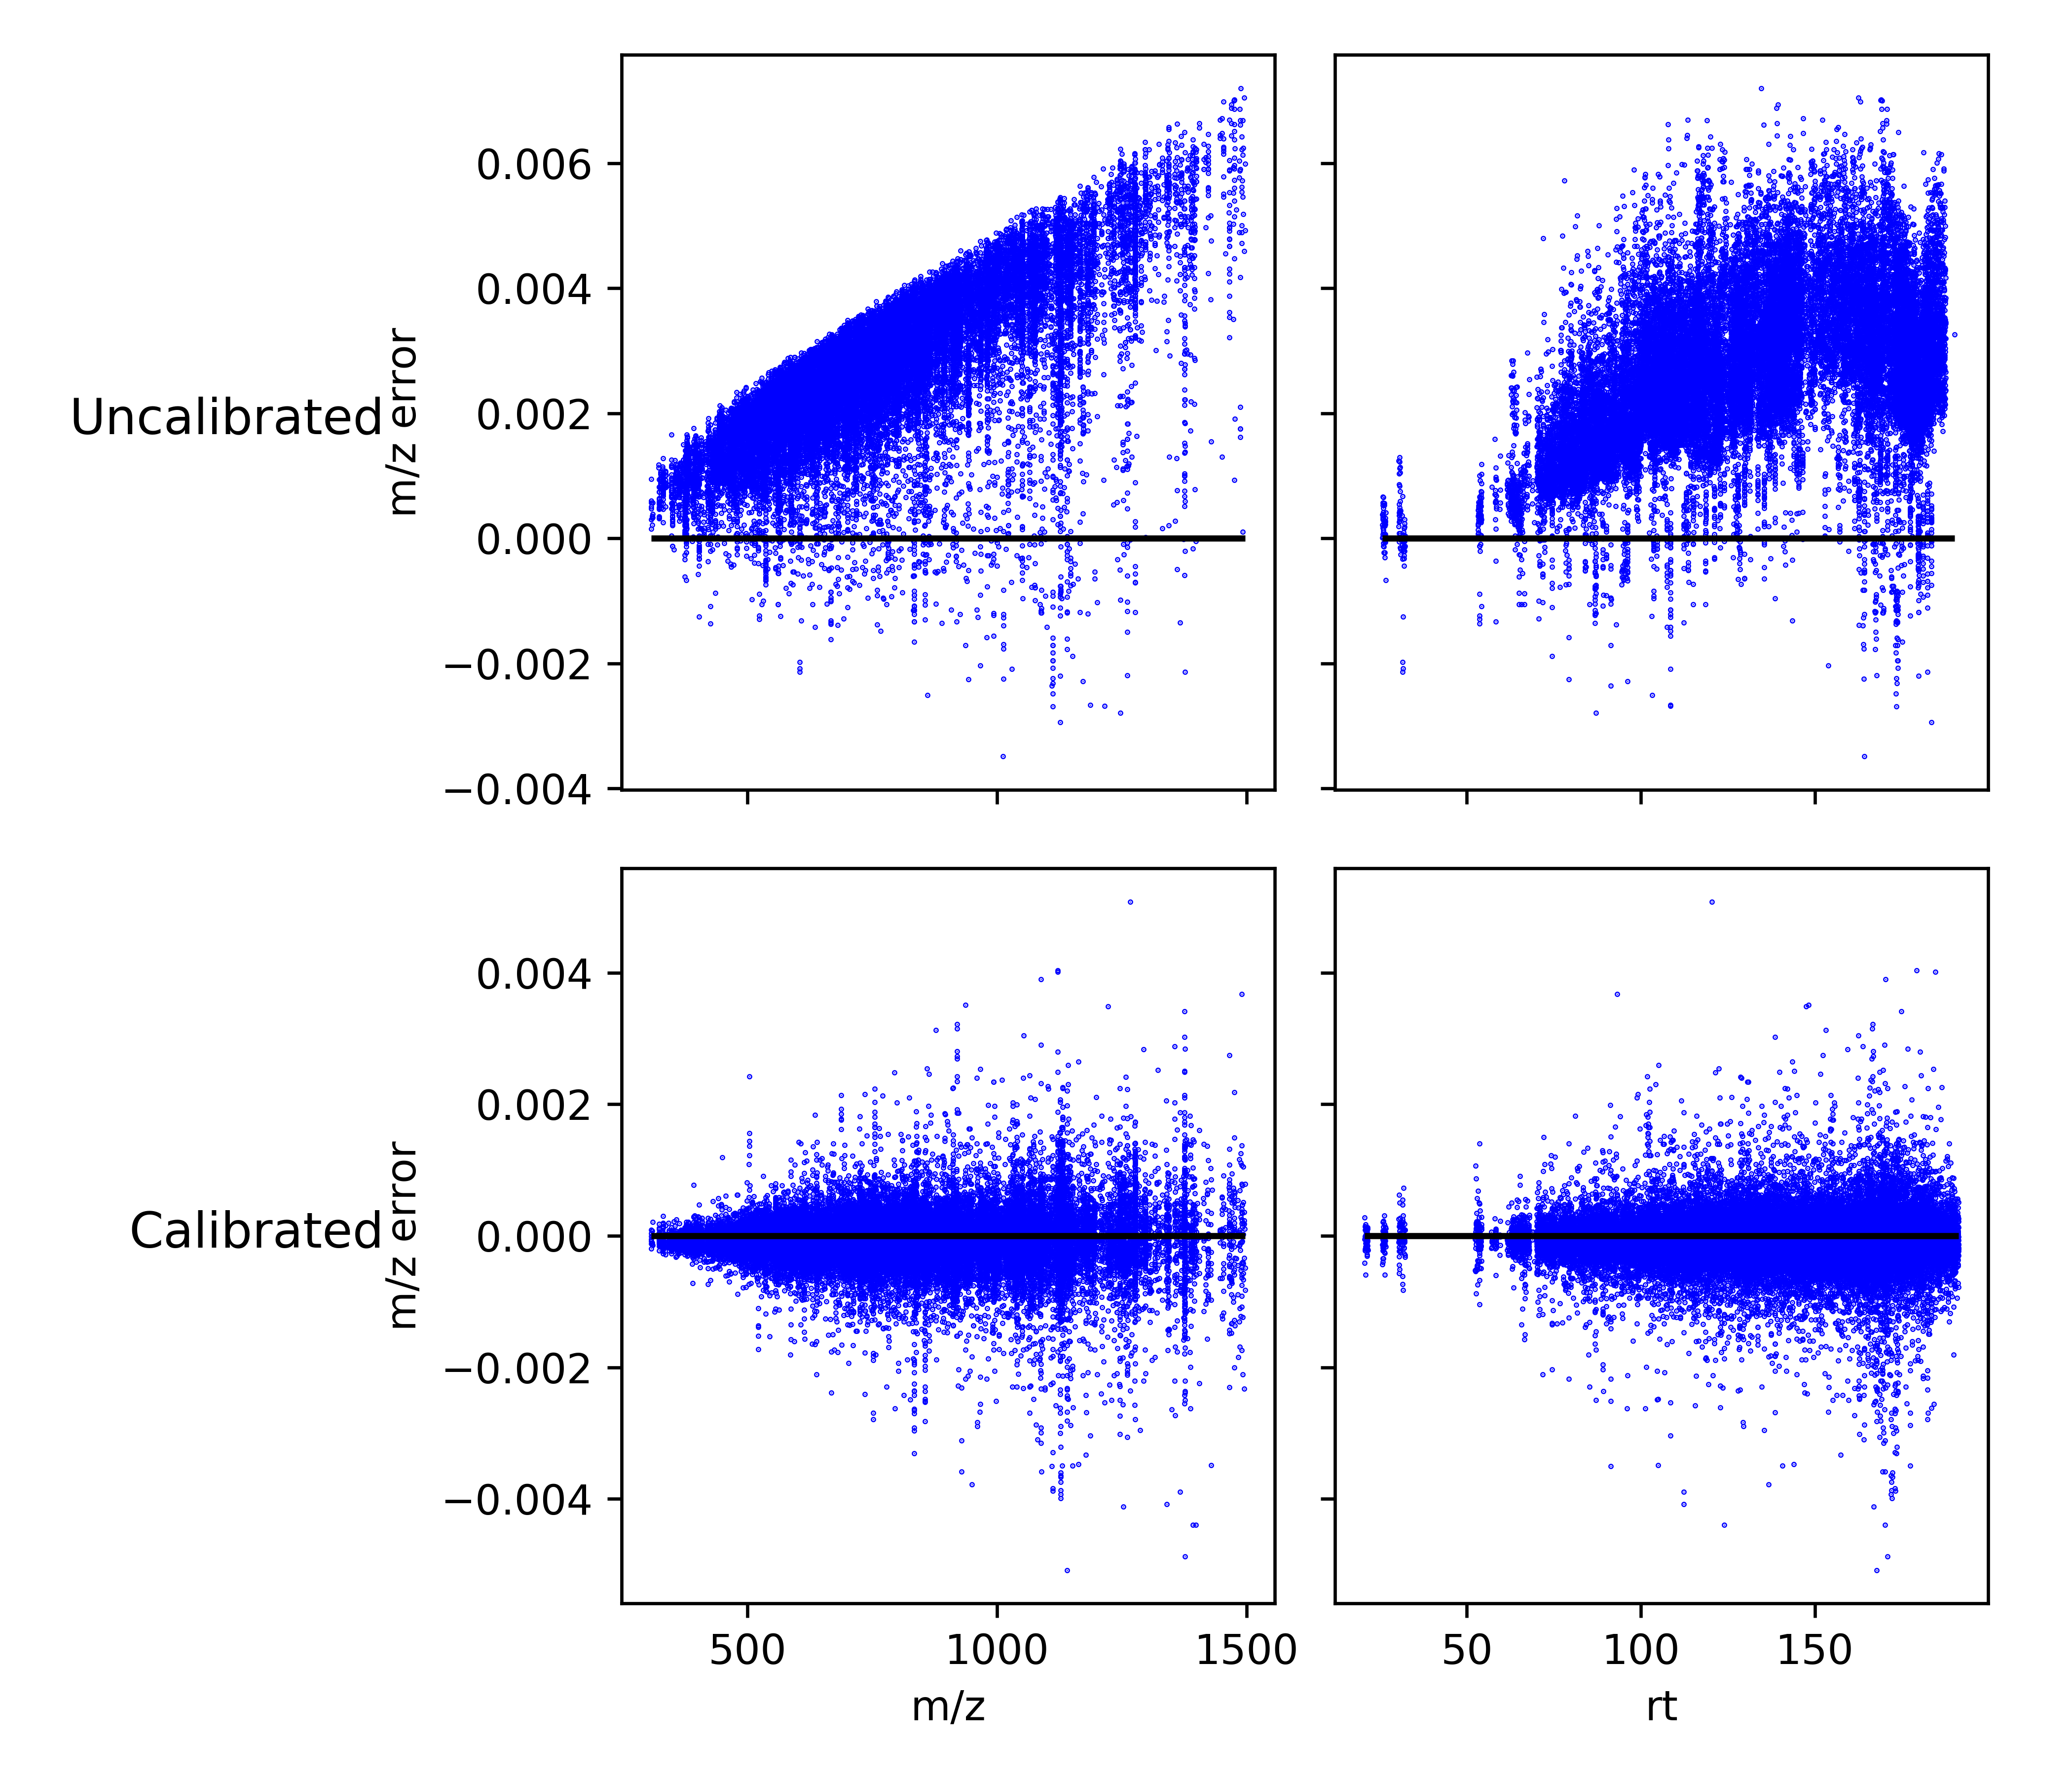
\includegraphics{fig1-calibErrors.png}
 \caption{Errors in m/z plotted vs the m/z value and the retention time}
 \label{fgr:fig1-calibErrors}
\end{figure}

Calibration quality improvements are also shown by the results of a standard database search, conducted on uncalibrated versus calibrated spectra using a 10 ppm precursor mass tolerance.
Table~\ref{tbl:calib} details the results of these searches.
The calibration procedure successfully addresses instrument miscalibration by centering the mass errors around zero ppm.
The systematic noise introduced by various other factors has also been corrected, as evidenced by the decrease in the standard deviation of the errors in the precursor masses, which shows that the calibrated mass spectra predominantly have sub-ppm mass errors.
A beneficial side effect of calibration is a corresponding increase in the number of confidently identified PSMs by around 1\%, when using the same wide 10 ppm precursor mass tolerance.
Histograms of the mass errors in identified peptides before and after calibration are plotted in Figure~\ref{fgr:fig2-10ppmSearchCalib}.
In summary, the main results of calibration are: more PSMs at 1\% FDR, decreased error in precursor mass, and decreased standard deviation in average mass error.

\begin{table}[]
\centering
\caption{PSMs Within 1\% FDR Before and After Calibration}
\label{tbl:calib}
\begin{tabular}{lll}

                                                                                      & Orig        & Calib        \\
 PSM Count                                                           &      217612   &   219172        \\
 Average Error (ppm)                                                              &      -2.10      &        -0.16      \\
 St. Dev of Error                                                    &       2.15      &        0.91      \\
\end{tabular}
\end{table}

\begin{figure}[H]
 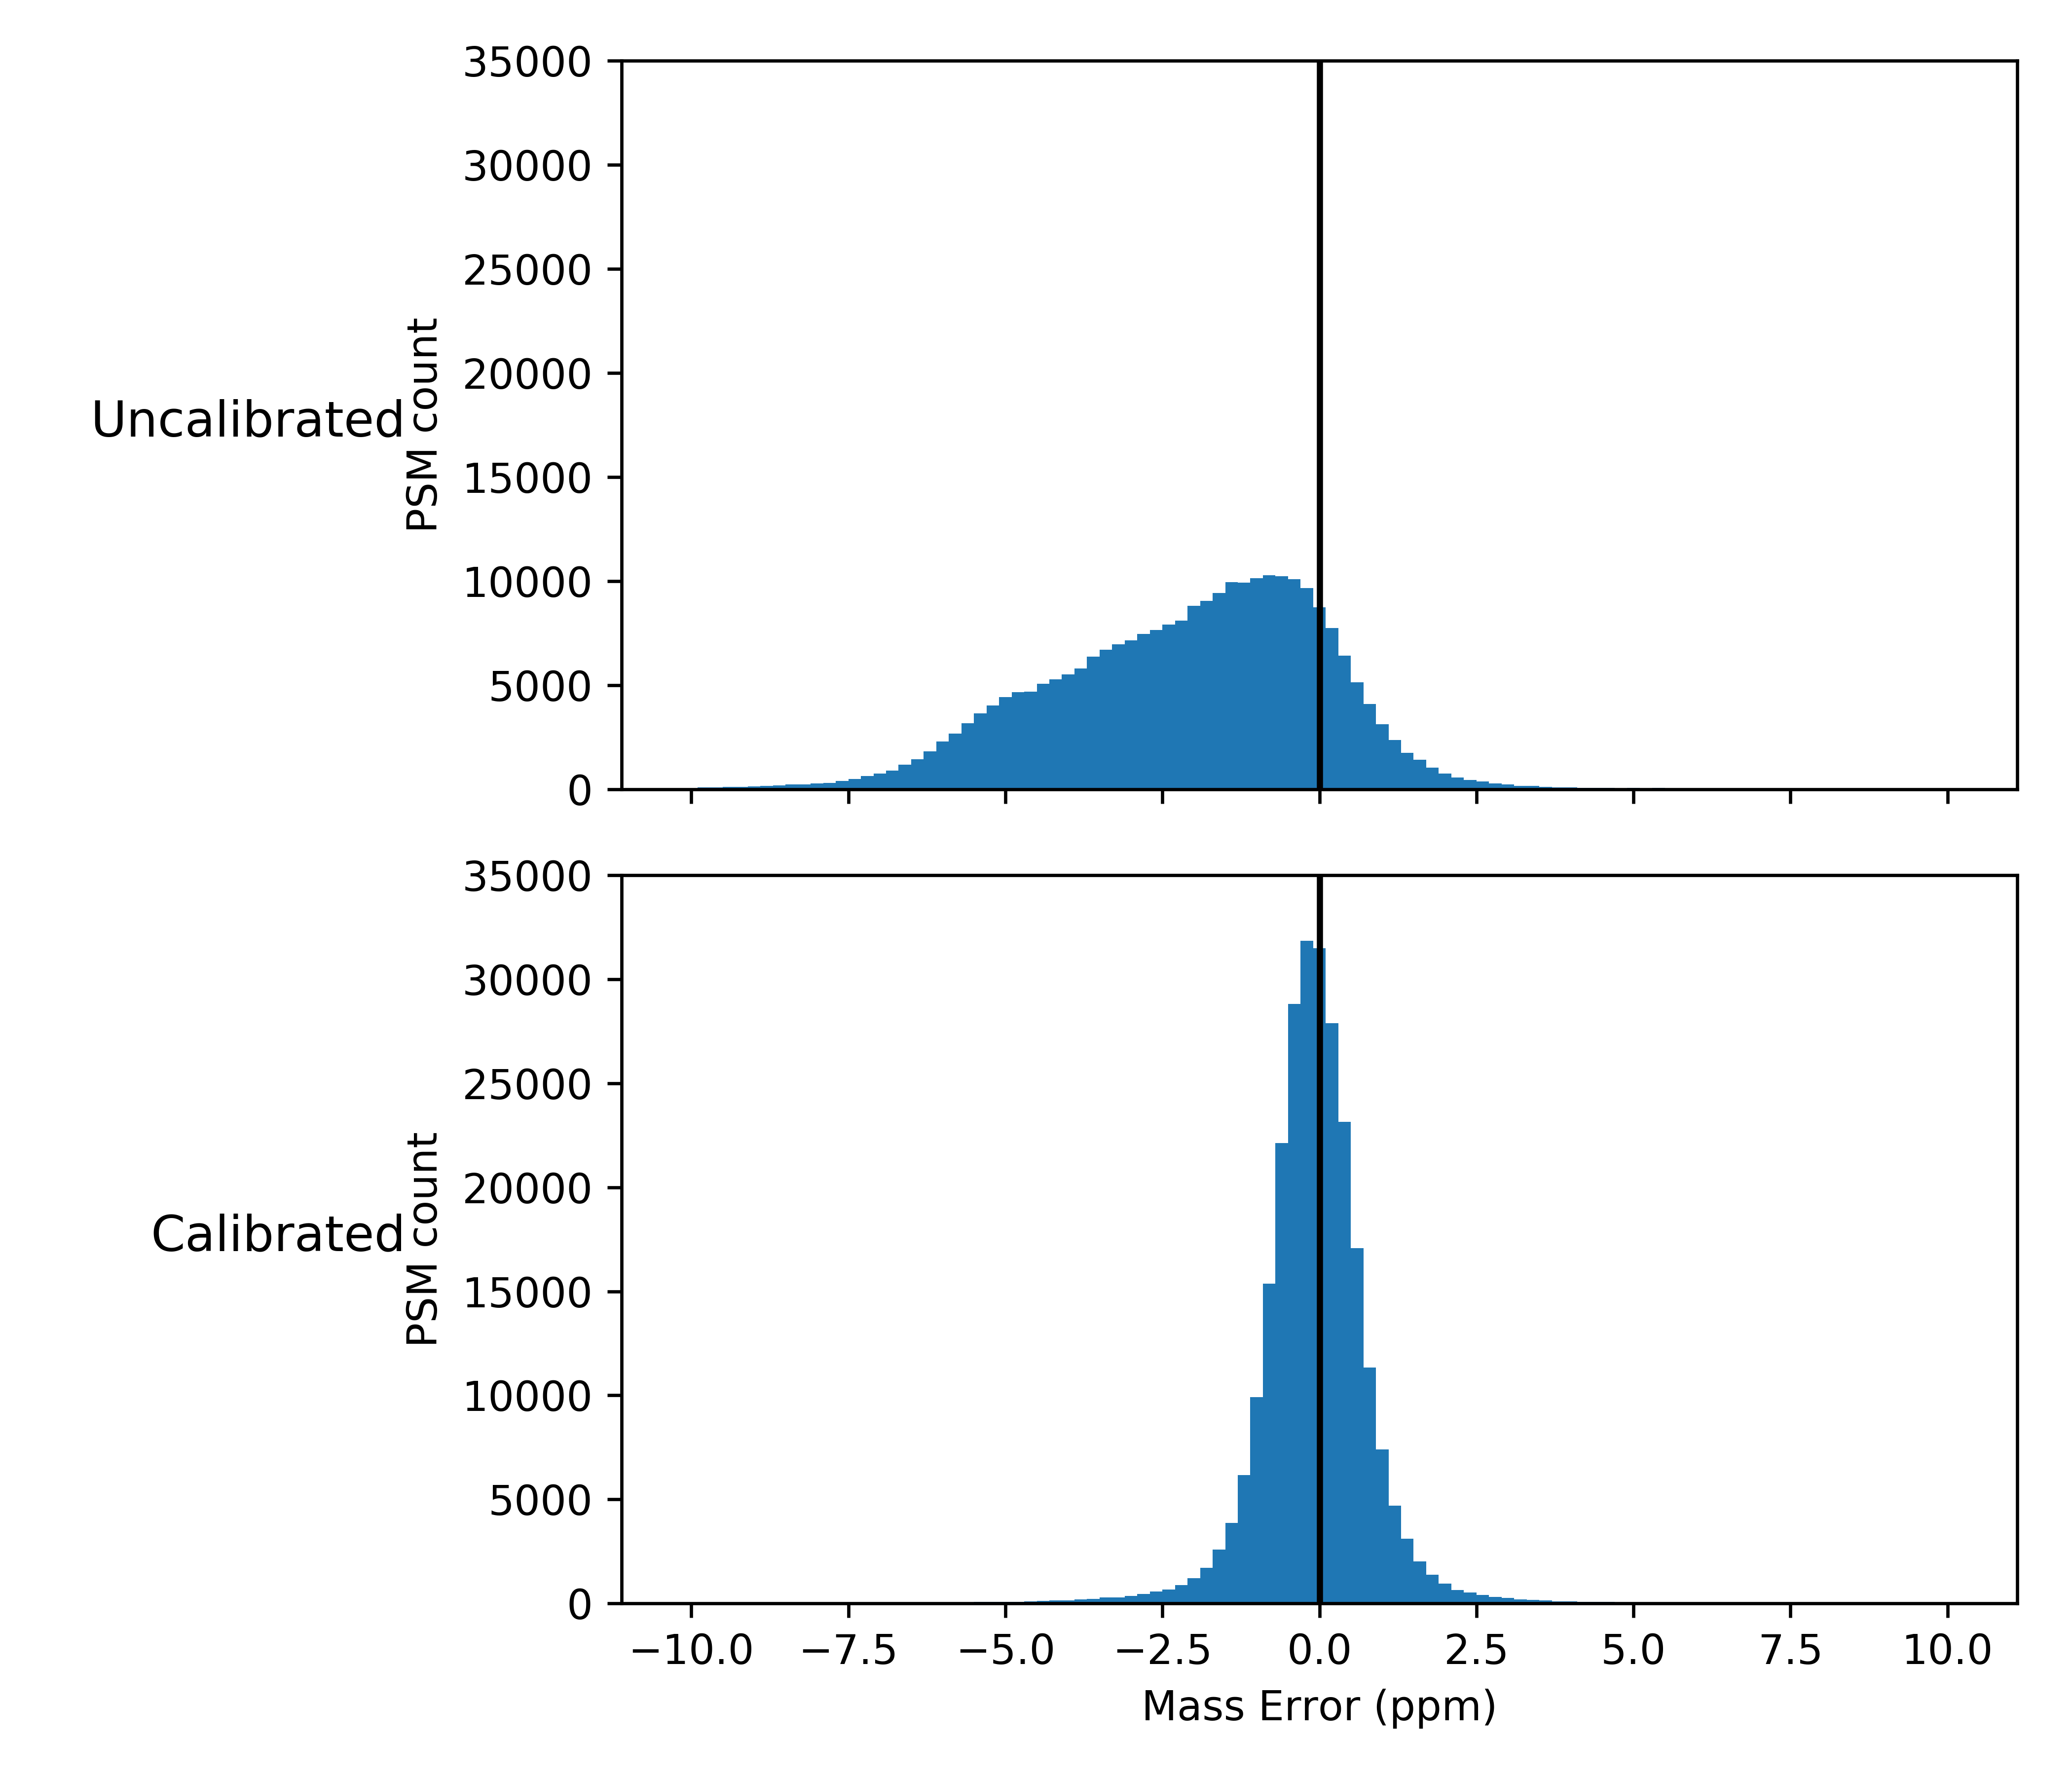
\includegraphics{fig2-10ppmSearchCalib.png}
 \caption{Histograms of the mass errors in identified peptides before and after calibration}
 \label{fgr:fig2-10ppmSearchCalib}
\end{figure}

\newpage

\subsection{Multi-Notch Searches}

It is useful to carefully describe the two commonly used database search approaches, prior to defining multi-notch searches and the impact that they have on G-PTM-D performance.
A traditional narrow-window search in bottom-up proteomics considers potential matches between theoretical peptides and experimental spectra if the candidate peptide mass and the observed precursor mass are equal within some defined tolerance (e.g. 5ppm, or 2.1 Da).
The other common search is an open search (e.g. $\pm 500$ Da)\citep{Chick_2015,Kong_2017,Li_2016}.
In searches of that type, the precursor mass and the mass of the best matching theoretical peptide could be many Da apart.
We describe an alternative to these search modes: the \textit{multi-notch} search.
This search is an extension of the narrow-window search that allows a variety of multiple specific mass differences between precursor mass and theoretical mass (See Figure~\ref{fig:fig3-searchTypes}) where the mass difference is easily interpretable.
It can also be seen as a narrowing of the open search to only allow prespecified mass differences.
The advantages and disadvantages of this alternative strategy are described below.

\begin{figure}[H]
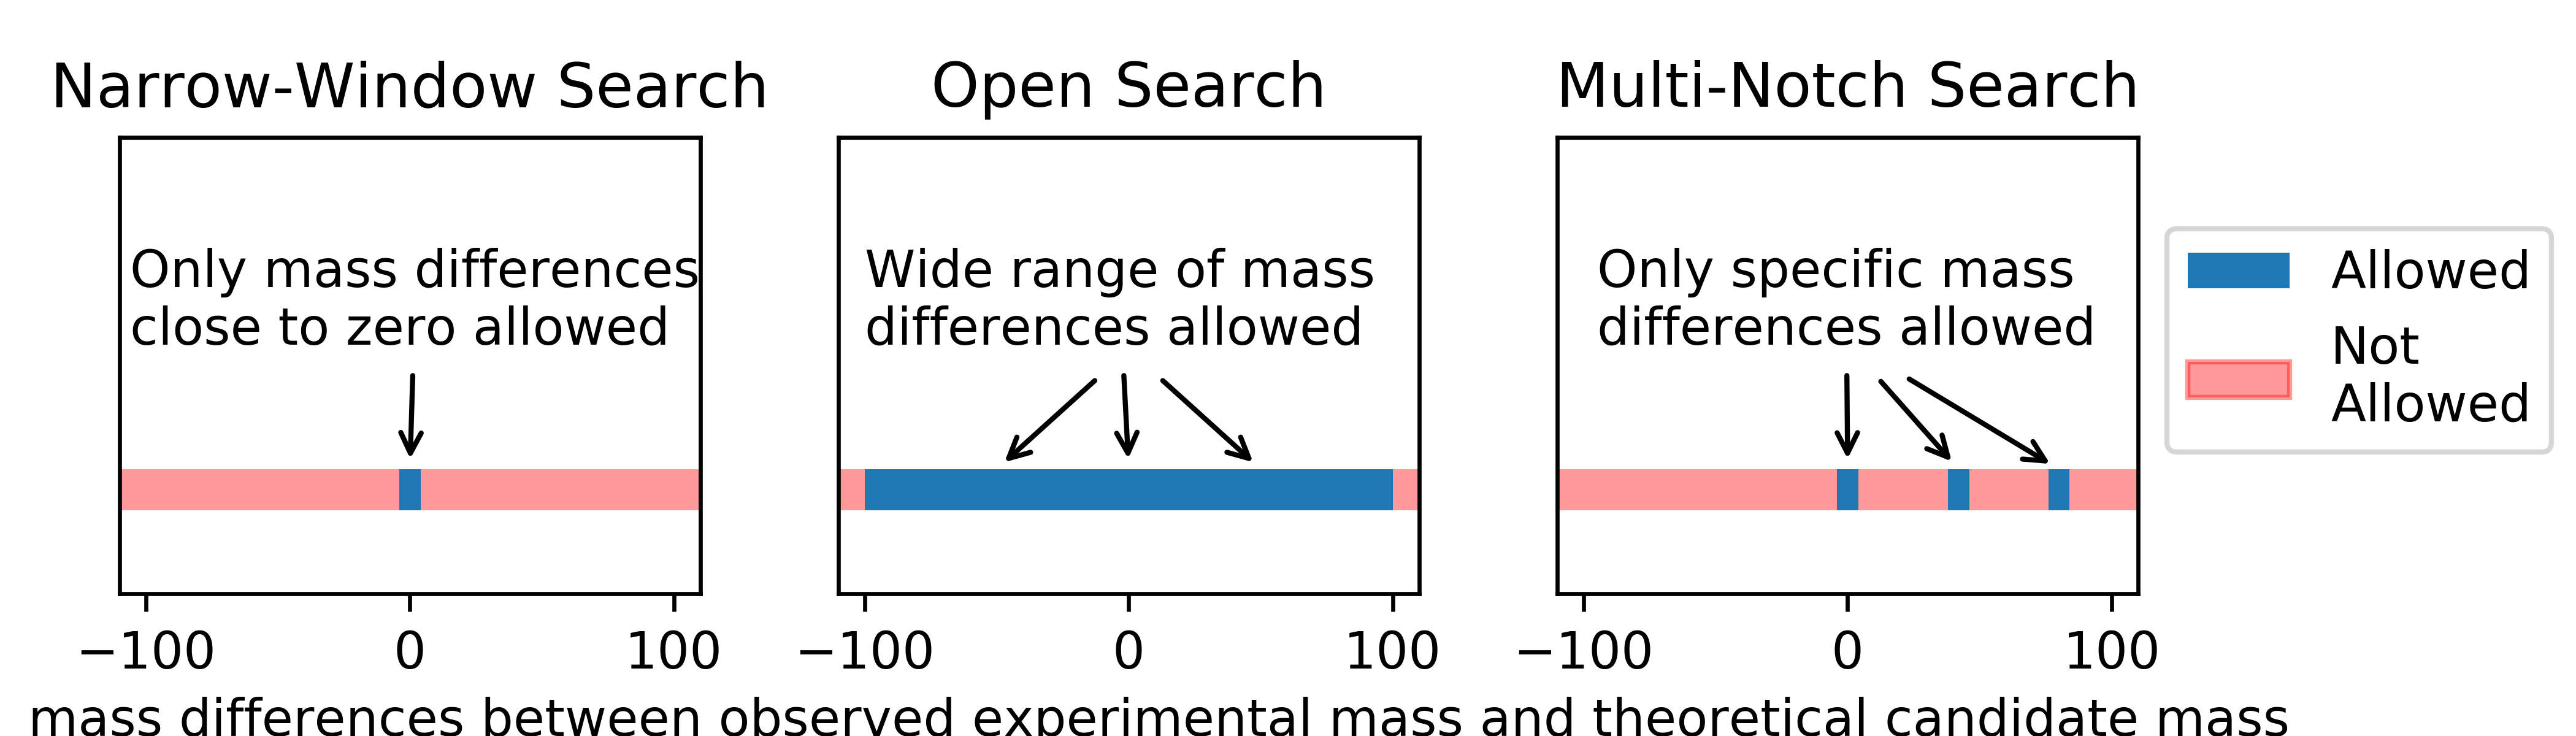
\includegraphics{fig3-searchTypes.png}
\caption{Search Modes}
\label{fig:fig3-searchTypes}
\end{figure}

\subsubsection{Traditional Narrow-Window Search vs. Limited Multi-Notch Search}

The traditional narrow-window search limits the range of acceptable mass differences between a candidate peptide and the observed experimental precursor in order to find an exact match to the observed peptide in a protein database.
A mass tolerance of <20ppm is commonly used on high-resolution MS1 data, resulting in a highly restrictive search.
It is not uncommon for the precursor mass tolerance of narrow-window searches to be relaxed to as much as 2 or 3 Da.
One rationale for this is that errors in the deisotoping of MS1 spectra frequently result in a reported experimental precursor mass being different by 1.0029 or 2.0054 Da from the true isolated peptide mass.
The relaxed tolerance approach identifies those peptides correctly.
A second rationale for this approach is that multiple peptides are frequently co-isolated and co-fragmented with all peptide fragments being observed in the same tandem mass spectrum.
Frequently, the best-fragmented peptide is different from the one corresponding to the precursor mass reported by the instrument, and the relaxed tolerance approach may identify this peptide, provided the reported charge state matches.
The major limitation of this approach is that a 2 or 3 Da tolerance includes mass shifts that, when present, may indicate that the matched peptide is not the correct identification, arguably defeating the purpose of a narrow-window search.
This may happen when the mass difference arises due to the identified peptide being different from the actual isolated precursor by a low mass modification or amino acid substitutions.

The described issues are apparent in mass difference histograms in Figure~\ref{fig:fig4jurkat-1012}, generated by compiling the results of a 2.5 Da tolerance narrow-window search.
These plots clearly show that numerous peptides have missed monoisotopic (Mm) peaks, deamidation, or an amino acid substitution.


\begin{figure}[H]
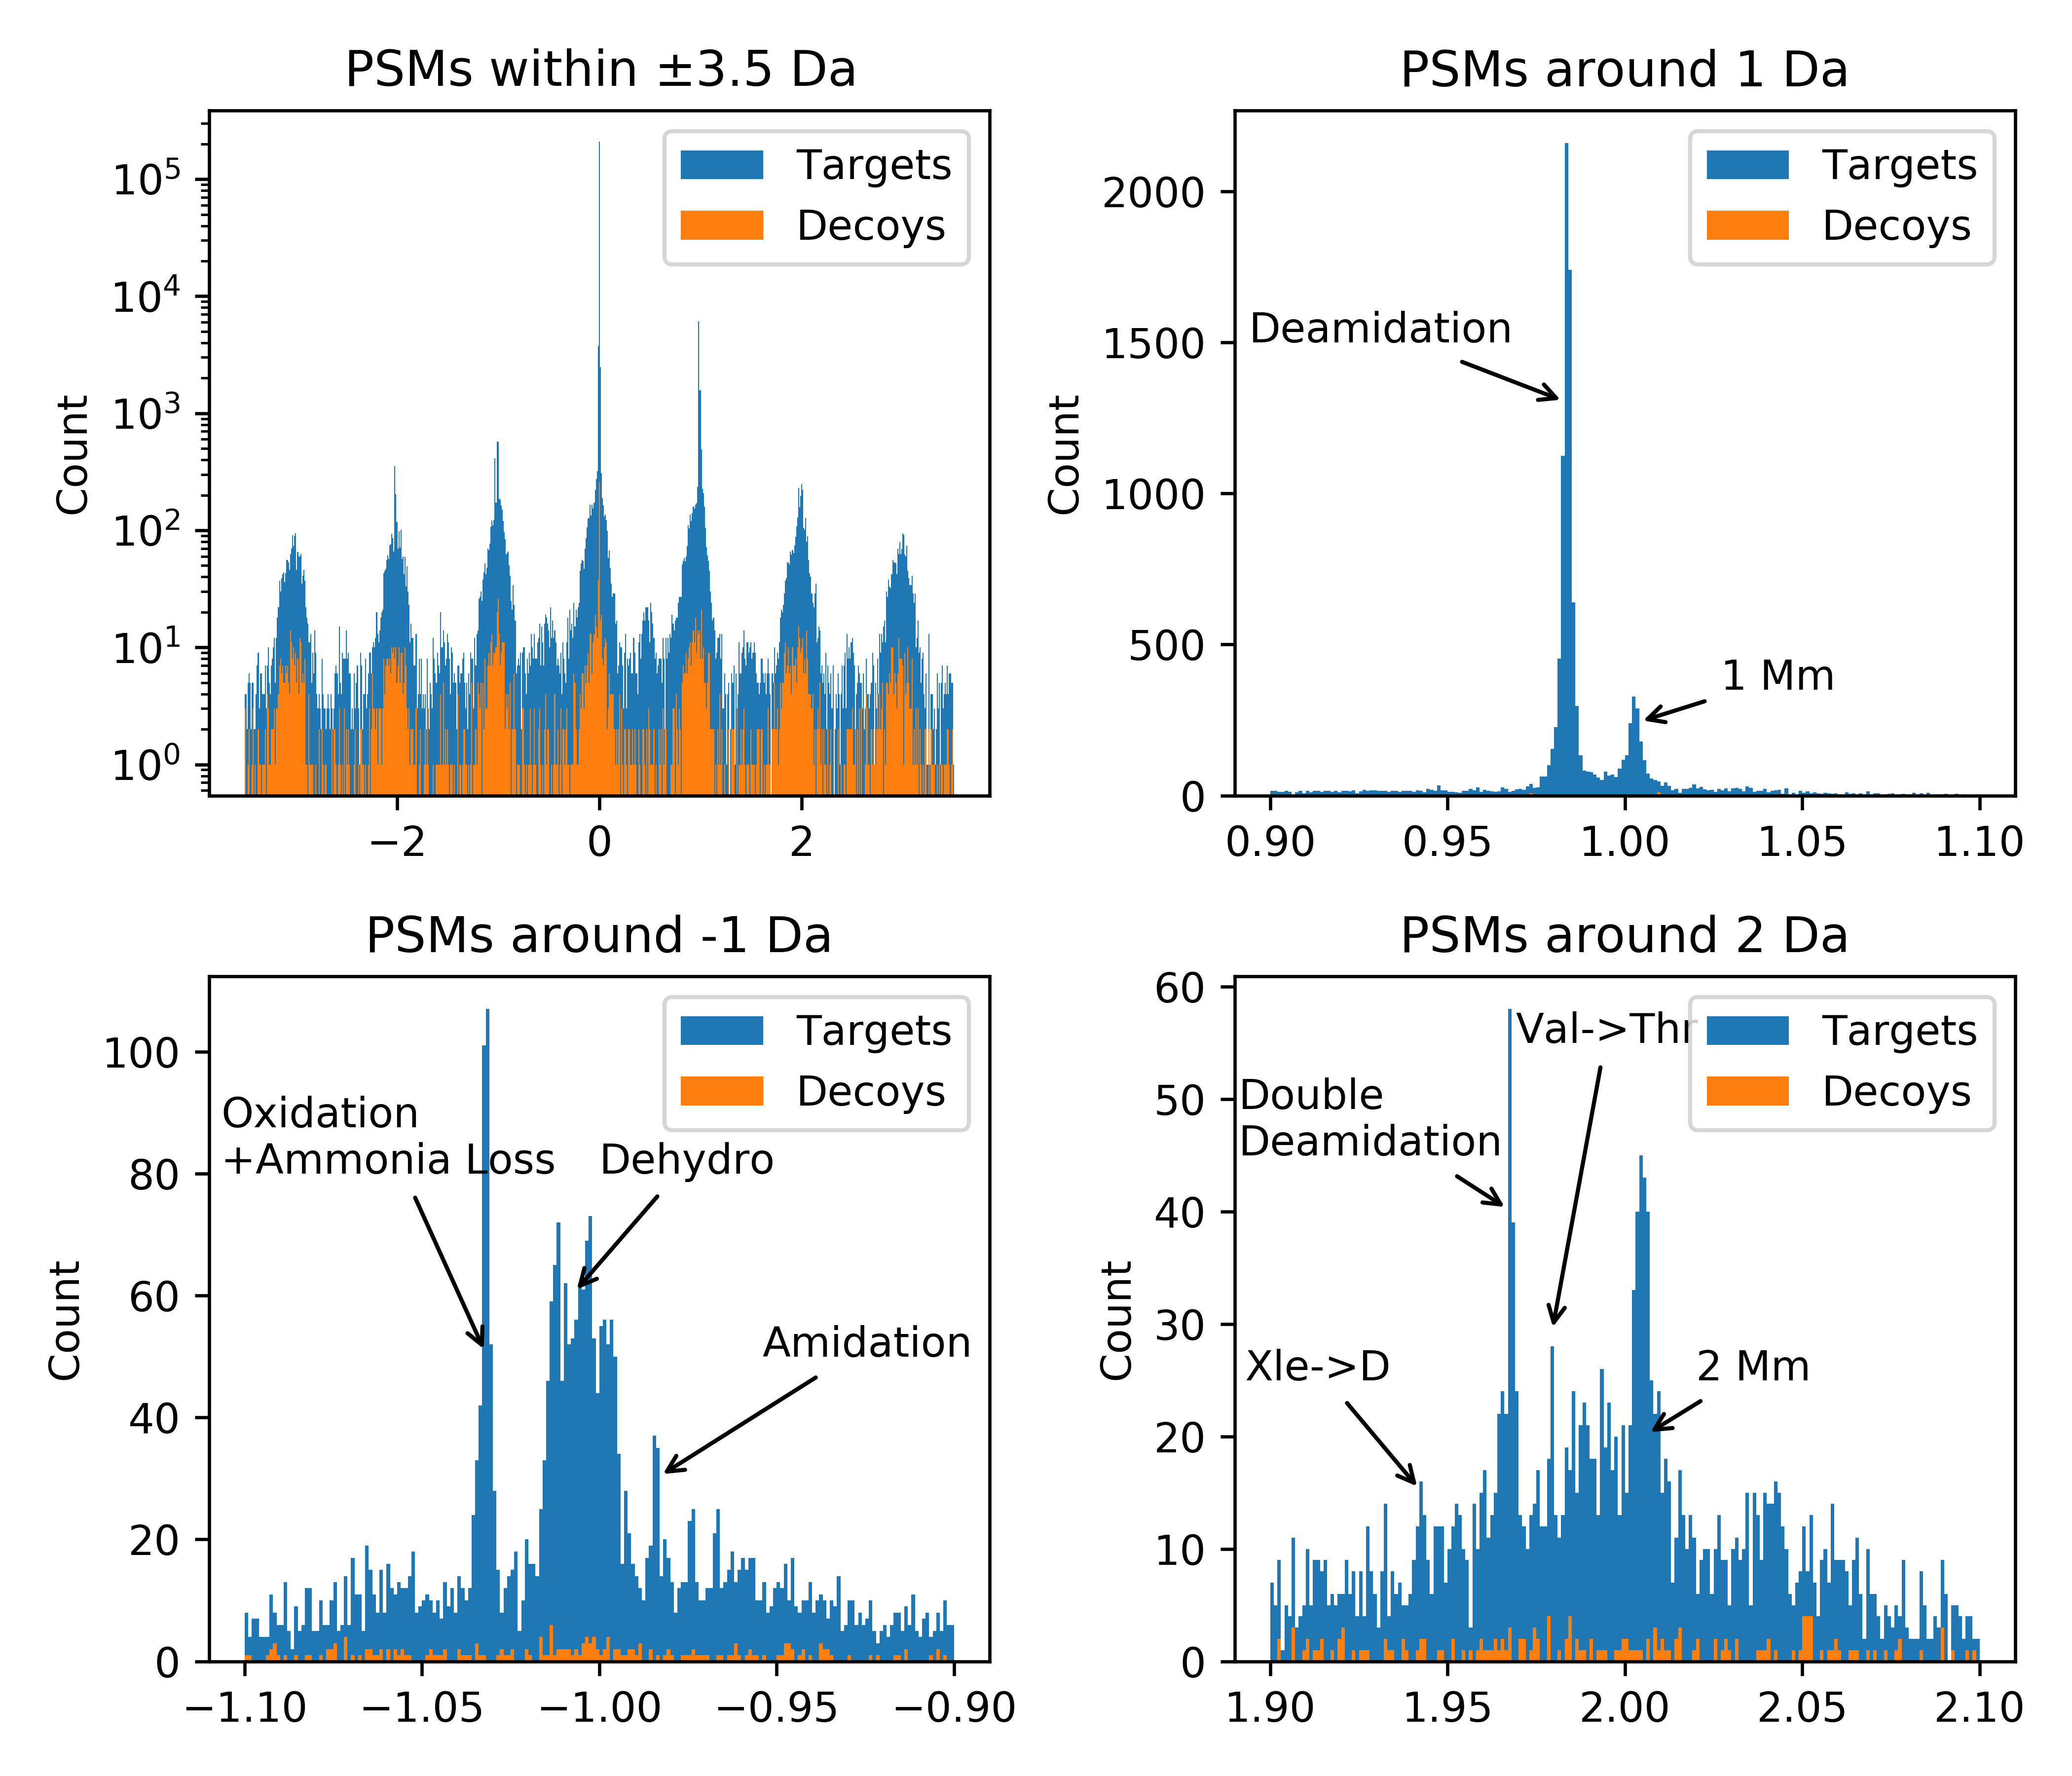
\includegraphics{fig4jurkat-1012.png}
\caption{Histograms PSM mass differences found in various dalton ranges}
\label{fig:fig4jurkat-1012}
\end{figure}

We propose a limited multi-notch search as a remedy to the trade-offs caused by choosing a narrow (few ppm) or wider (few Da) precursor mass tolerance during a traditional narrow-window search.
This limited multi-notch search allows mass differences between precursor and theoretical peptides of 0, 1.0029 and 2.0054 Da, but it limits the width around these three mass differences to a few ppm (1-20 ppm).
This approach provides a means of getting an increased number of correct identifications while mitigating problems with incorrect identifications.
This alternative would appear to result in loss of identification of co-isolated peptides, but MetaMorpheus is programmed to handle this problem by identifying multiple co-isolated precursor masses (see section below).

To illustrate the described advantages, we compared the three types of searches using all 28 calibrated Jurkat fractions (Table~\ref{tbl:singleVsMultiNotch}).
The limited notch search yields the largest number of confidently identified PSMs with only a small fraction being misassinged.
We consider PSMs to be misassigned if the G-PTM-D procedure determines a higher-scoring modified peptide for a PSM, see the last section for details.

\begin{table}[]
\centering
\caption{Notch Search vs Narrow-Window Search comparison of PSMs for Mouse}
\label{tbl:singleVsMultiNotch}
\begin{tabular}{llll}
                    & 5ppm Search & 2.5 Da Search & Notch Search \\
PSMs Within 1\% FDR & 275359      & 262543        & 279895       \\
misassigned PSMs    & ?           & ?          & ?            \\
\end{tabular}
\end{table}

A specific example of a misassigned PSM is the example where the correct identification has oxidation and ammonia loss, but was identified as an unmodified peptide with score 9.039 and mass difference of -1.03335 Da, with sequence QAFDDAIAELDTLNEDSYK, Jurkat Frac9 scan 20962.
With G-PTM-D added modifications, the correct peptide is identified with sequence [PeptideTermMod:Ammonia loss on Q]QAFDDAIAELDTLNEDSY[Mod:Oxidation on Y]K. It has a mass difference of -0.00171(-0.79458 ppm) and a score 19.222.

\newpage

\subsubsection{Multi-Notch Search vs. Open Search}

Chick et al. showed that by significantly relaxing the precursor mass tolerance in bottom-up searches, an incredible variety of unforeseen peptides were being fragmented and could be identified\citep{Chick_2015}.
In particular, PTM-containing peptides could be identified from those MS2 fragments that did not possess the modification and the type of PTM could be inferred from differences in identified peptide mass and precursor mass.
A major limitation of the Chick work was the extremely long search times because of the vast number of theoretical candidate peptides that were evaluated for each and every MS2 spectrum.
Recently, Kong\citep{Kong_2017} reported a new index-based search strategy (MSFragger) that radically improved search speeds for open searches.
Search times for $\pm 500$ Da precursor tolerance went from six years to six seconds.
The output of both search strategies is a list of PSMs, where the best matching unmodified theoretical peptide was found for each MS2 fragmentation spectrum and the mass difference between the theoretical and experimental precursor masses was determined.
The mass differences can be clustered into histogram peaks\citep{Rodriguez_2014}, with interpretation of the mass difference left as an exercise for the user.

There is a major problem with using the results from unrestricted precursor mass tolerance searches to infer peptide modifications regardless of whether they are of the Chick or Kong variety.
The freedom in precursor mass difference results in a multitude of false positive \textit{mass difference identifications}.
For example, small missed cleavages are often reported as mass differences.
The peptide PEPKK is often identified as PEPK with a mass error of 128 Da (the converse is also true, PEPK may be identified with a mass error of -128 Da).
This error is relatively easy to spot but when the missed cleavages contain multiple amino acids, the interpretation and discovery of the error is much more difficult.
Another example of this relates to peptide modifications.
The phosphopeptide PEPpSK could be reported with a mass error of -79.96 Da when the better identification would have been PEPSK.

The alternative we recommend, is the use of a multi-notch search, which offers a means of reducing the search space and limiting the number of theoretical candidates to those plausible for the scan, increasing the search speed and most importantly, producing the most correct PSMs with the fewest false positive PSM identifications.

We compared searches of all Jurkat fractions using a $\pm 500$ Da wide mass search versus a multi-notch search with notches at 0 and 79.961 with 0.02 Dalton tolerance.
The advantage of the multi-notch search over the open search is shown in Table~\ref{tbl:multiVsWide} by at least a $10\%$ increase in the number of target PSMs with score of at least 9.079, for both regions (0 Da no-PTM peptides and +79.96 Da phosphorylated and sulfonated peptides).
It is important to point out that the difference in the numbers of PSMs is not due to FDR considerations, but rather to the erroneous peak assignment in open searches.

\begin{table}[]
\centering
\caption{Multi-Notch Search vs. Open Search}
\label{tbl:multiVsWide}
\begin{tabular}{lll}
                    & Open & Multi-Notch\\
0 peak    & 176073  (0.15\% FDR)     & 193328 (0.23\% FDR)     \\
79.96 peak     & 732   (0.68\% FDR)   & 957  (0.84\% FDR)           \\
\end{tabular}
\end{table}

The same results are presented in a graph format in Figure~\ref{fig:fig6-ZeroAndPhospho}.

\begin{figure}[H]
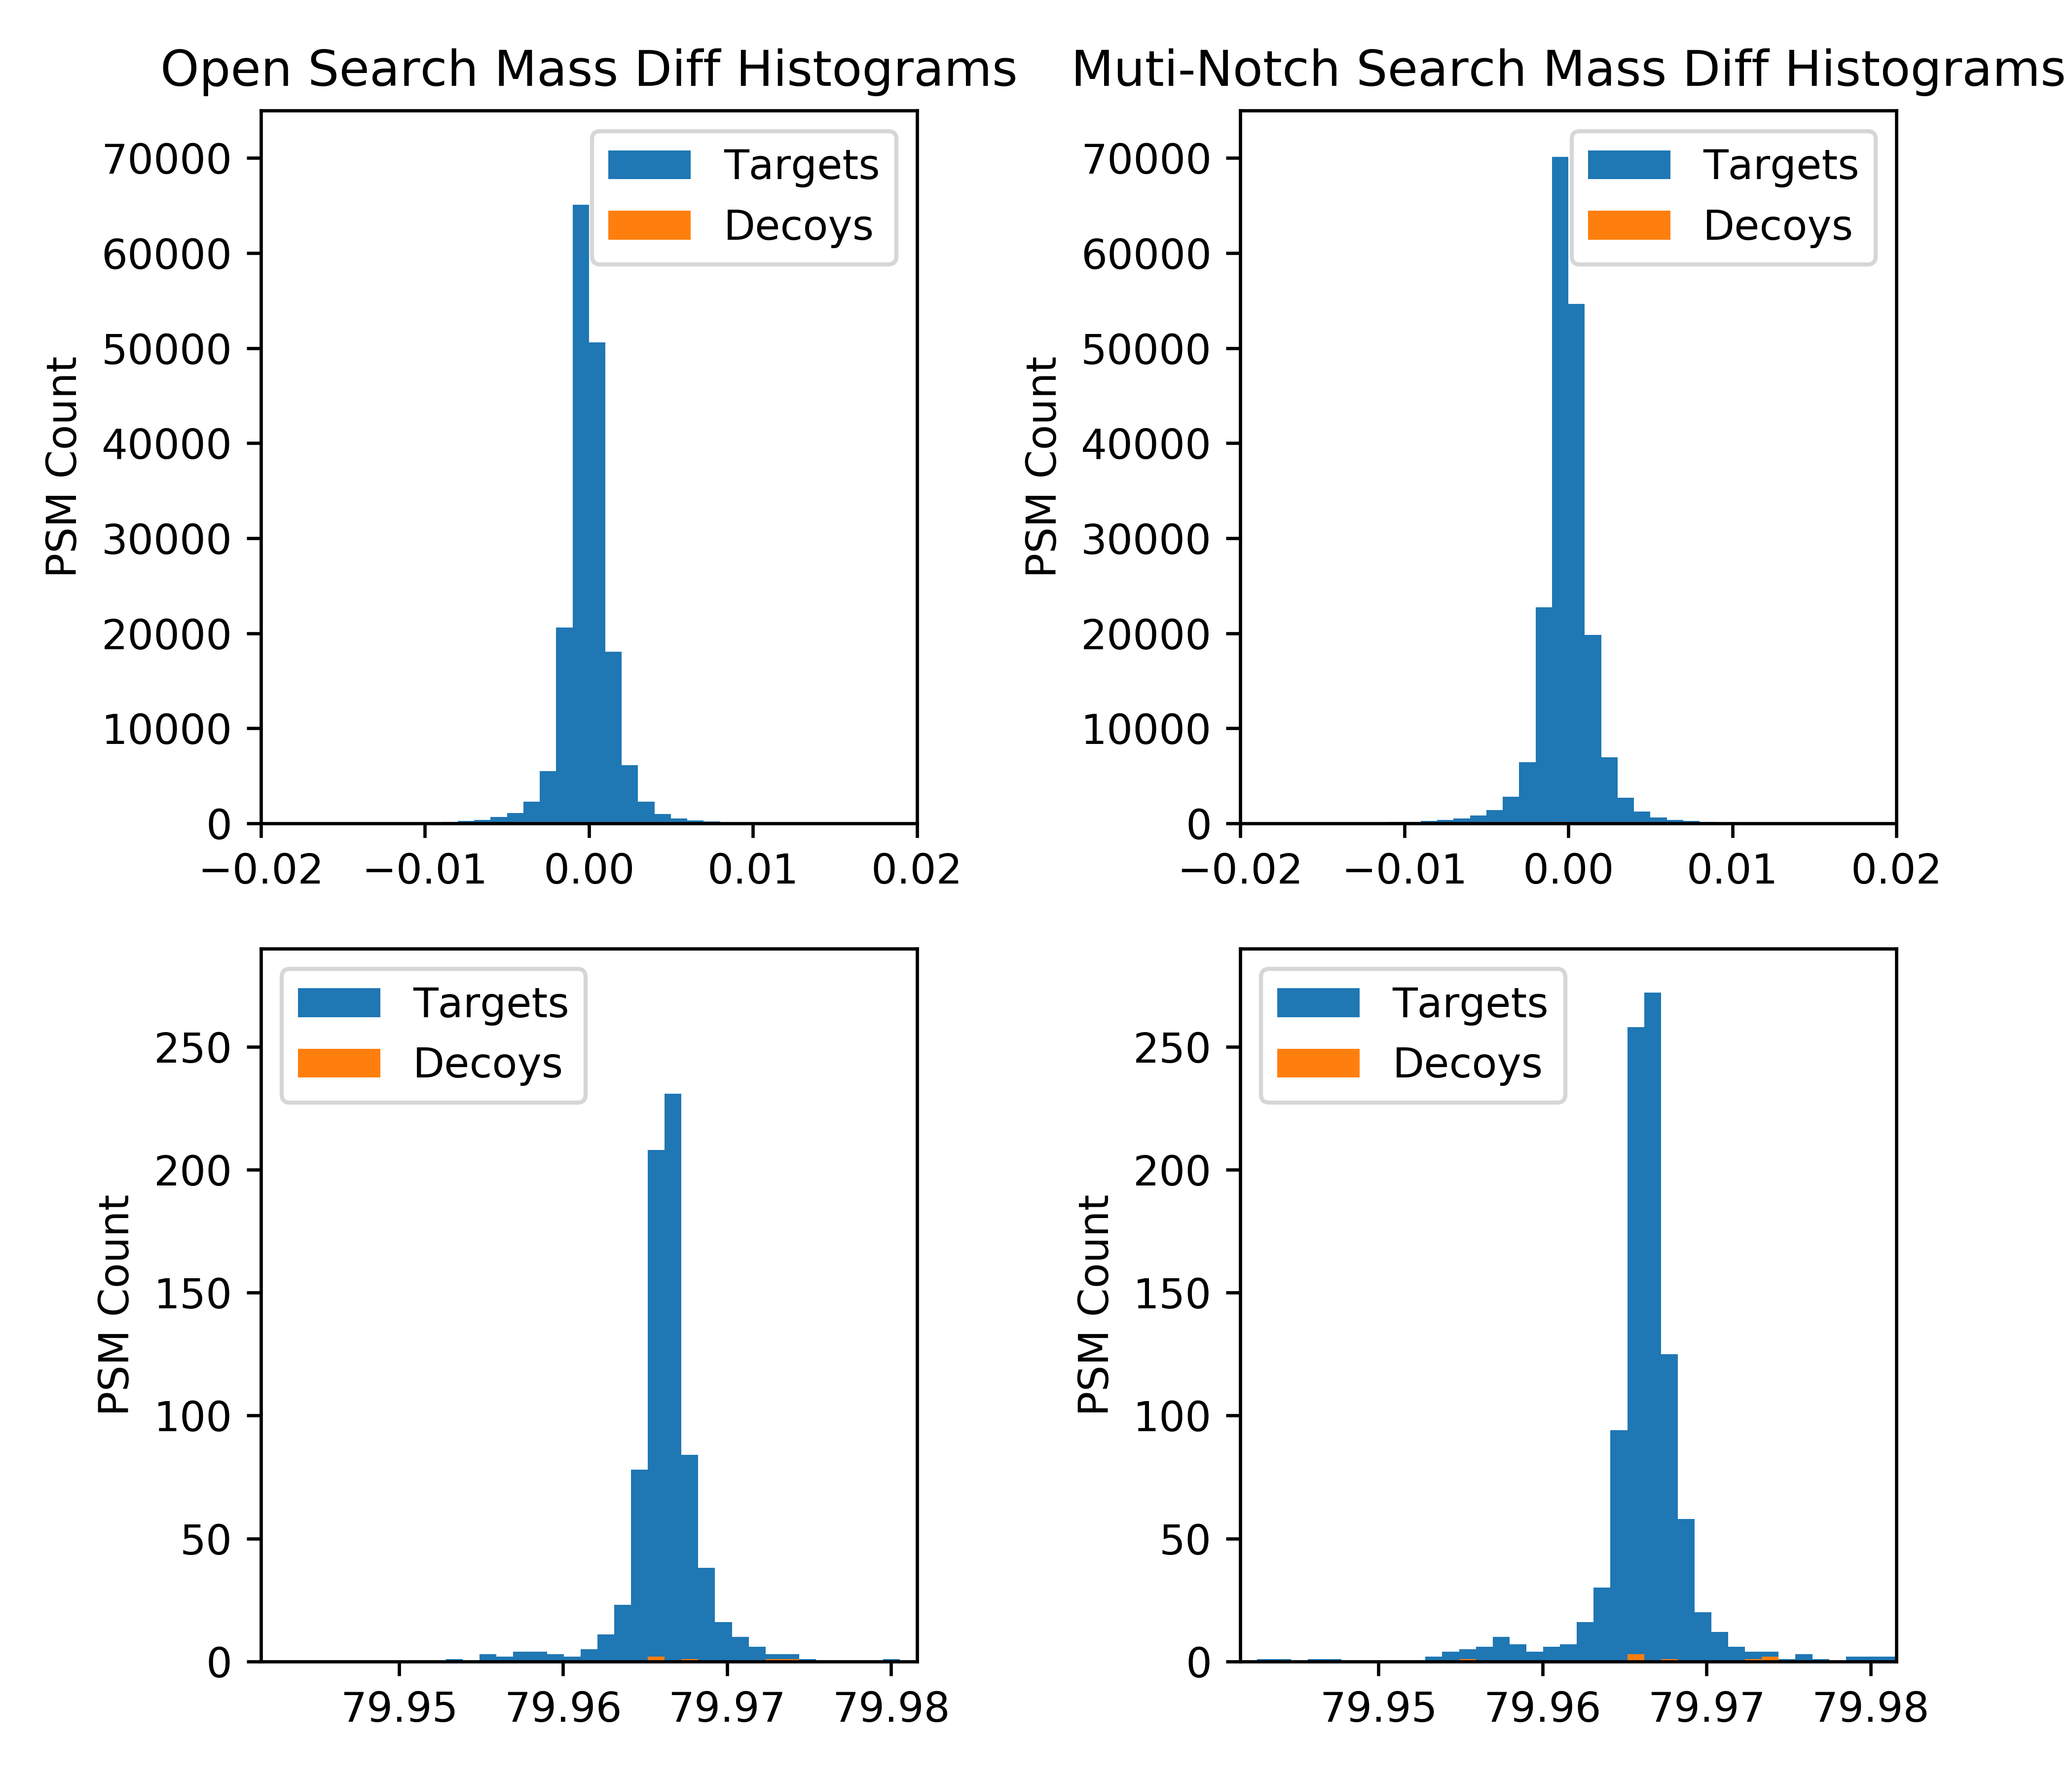
\includegraphics{fig6-ZeroAndPhospho.png}
\caption{Zero and Phoshpo and Sulfo}
\label{fig:fig6-ZeroAndPhospho}
\end{figure}

A specific example of a PSM that has been erroneously assigned in a open search is scan 12835 in Jurkat frac 5.
The open search identifies ATPARAPESPPSADPALVAGPAEEAEC[Common Fixed:Carbamidomethyl of C]PPPR as the best match with a score of 17.231 and mass difference of -416.31028, and a single missed cleavage.
The identified b ion matches are 172.08479,269.13756,880.44028.
The better match is identified by the multi-notch search, as APESPPSADPALVAGPAEEAEC[Common Fixed:Carbamidomethyl of C]PPPR with a score of 16.246 and mass difference of 79.9655, and no missed cleavages.
The identified b ion matches are 168.08988,297.13247.
So, instead of having a PSM with an unidentifiable mass shift of -416.31028 (mass of removal of ATPAR and addition of phosphorylation), we have an easily identifyable mass shift corresponding to a phosphoyrlation site.

\subsection{Co-isolation}


Consider the scan JurkatFrac12 scan 12336. Isolation m/z  = 726.65.
Isolation width is 2.5 Th.
It is shown in Figure~\ref{fig:fig5-coIsolationSpectrum}.


\begin{figure}[H]
\includegraphics{fig5-coIsolationSpectrum.png}
\caption{m/z peaks in scan 12333}
\label{fig:fig5-coIsolationSpectrum}
\end{figure}

We showed above in Figure~\ref{fig:fig5-coIsolationSpectrum} an example where several peptides were co-eluting from the column into that mass-spec within the tolerance used for isolation for fragmentation.
In that particular case, the precursor with m/z 726.65 was chosen for isolation and fragmentation.
In a conventional search, only that precursor mass would be used to select a range of theoretical for comparison.
However, all peptides in that range are co-fragmented and a better solution would be to use all co-isolated precursor masses.
In MetaMorpheus, for each MS2 scan, the corresponding MS1 scan is deconvoluted and the complete list of precursors is gathered for the range surrounding the isolated precursor ($\pm 1.25$ Th).
Each deconvoluted mass is used to select a range of theoreticals to use for identification.
The result of this is that often, more than one peptide can be identified from a single MS2 scan.
Below, in Table 3434, we should the number of PSMs for a raw file where we use only a single precursor mass and we compare that to the case where we allow for multiple different precursors.
You can see a significant increase in the number of identified PSMs.
Importantly, you can see in Supplemental Figure erf3e, that the precursor mass errors go down significantly and the standard deviation is much reduced.
This is extremely beneficial in both open mass and multi-notch searches because it reduces the number the more difficult to interpret mass shifts and substantially improves G-PTM-D (see below).

Get the story about how precurors with similar m/z with different z can in their deconvoluted state be many (10s, 100s of Da apart).
This is a big problem in general searches but also for open mass and multi-notch searches which are used to discover possible PTMs.

MetaMorpheus was programmed to ignore the precursor mass reported by the mass spectrometer in the mass spectrum and instead, deconvolutes all peaks in the MS1 spectrum associated with the tandem mass spectrum to recover all possible precursor masses.
This expanded list of precursors is used in every spectrum match, frequently resulting in multiple peptide identifications from single tandem mass spectrum.


\subsection{Enhanced G-PTM-D Results}

In the original G-PTM-D manuscript, an open mass search ($\pm 200-500 $ Da) was used to create a histogram of mass difference peaks, from which a number of PTMs could be inferred.
A Perl script was used to mine those mass differences to modify a proteomics database with potential PTMs.
This database was used for a final search and a number of PTMs were identified.
There were several limitations to that work.
One, the open mass search was really slow.
Two, uncalibrated data made it hard to discern closely spaced modifications.
Three, certain mass differences with high FDRs were incorrectly allowed.
Four, missed monoisotopic peaks and co-isolated peaks were not handled.
Five, separate programs were required (both Morpheus and a Perl script).
MetaMorpheus resolves all of these issues and more.
Below we will show how each individual enhancement to G-PTM-D improved performance over the original work and then we will show at the end, the combined effect of all enhancements.

A major improvement in G-PTM-D performance arises from using calibrated spectra as inputs to the procedure.
Calibration and the associated increase in mass accuracy is essential for discrimination of small differences between mass shifts due to different modifications.
To illustrate this, mass shifts around 80 Daltons from the initial notch search are aggregated in the histograms in Figure~\ref{fig:phosphoHistograms}.
It is evident from these histograms that the phosphorylation and sulfonation peaks are clearly separated and identifiable when the search is conducted on well-calibrated spectra.

[THERE IS SUPPOSED TO BE A COOL FIGURE HERE]

G-PTM-D originally added PTMs with masses that were included in the UniProt PTM list.
We have since greatly increased the variety of PTMs added by including a number of new notches in the G-PTM-D first pass search.
The new notches correspond to metal adducts (e.g. Na and K), glycosylations., sample handling and processing artifacts (e.g. carbamylation, ammonia loss), lipidation, and etc.
The improvement in accuracy and lowering of mass error were sufficient that many new modifications at large mass and many PTM combinations could be confidently added and discovered using the newly enhanced G-PTM-D approach.
We show, in TABLE/FIGURE below a list of PTMs used in the original G-PTM-D search along with the list of PTMs used in the enhanced G-PTM-D search.
The number of different modifications increased from 22 to 333.
The total number of PSMs increased by . We also show in the table the associated local FDR.

We identified peaks in the original G-PTM-D approach with anomalously high false discovery rates, which could be excluded from wide mass searches in order to improve the overall identification quality.
Some of these problematic histogram peaks are illustrated in Figure, including peaks corresponding to masses of sulfonation and phosphorylation, and a problematic peak at mass of Leucine, with a high FDR (see Table above).
INSERT A GREAT PLOT HERE We identified some specific mass shifts that are characterized by anomalously high false discovery rates: these mass shifts correspond precisely to various combinations of residue mass additions and removals.
MSFragger also doesn’t automatically calibrate spectra prior to searching.
Therefore, mass differences from closely spaced PTMs (e.g. phosphorylation and sulfonation) can easily be misinterpreted.
MetaMorpheus has built in functionality to identify multiple peptides from each tandem mass spectrum resulting in improved identification of peptides and peptide modifications.

By employing the novel multi-notch search strategy instead of the open search in the G-PTM-D process, using only the modifications listed in UniProt, the number of confidently identified PSMs increased by 6\%.
The overall search time dropped significantly, from 35 hours to 4 hours for all datasets, see Table~\ref{my-labelff}.

\begin{table}[]
\centering
\caption{Effects of Replacing Initial Wide-Mass Search by a Multi-Notch Search}
\label{my-labelff}
\begin{tabular}{ll|l|l}
                      &        & Wide-Mass Search & Notch Search\\
\hline
\multirow{2}{*}{Time} & Jurkat & 22.1 hrs         & 2.9 hrs    \\
                      & Mouse  & 13.5 hrs         & 1.2 hrs   \\
\hline
\multirow{2}{*}{PSMs} & Jurkat & 203237           & 210566    \\
                      & Mouse  & 153674           & 162473   
\end{tabular}
\end{table}


The final notch search uses notches centered at \{0, 1.0029, 2.0054\}, in order to capture missed identifications due to missed monoisotopic peaks.
The results are contrasted with the standard narrow-window final search.
The effect of using these notches is shown in Table~\ref{tab:table2}.

We observe that when using an incomplete database that does not include comprehensive modification and sequence variation information, a notch search with notches at monoisotopic peaks is superior to either of the narrow-window searches.

\begin{table}[]
\centering
\caption{Effects of Replacing Final Narrow-Window Search by a Notch Search}
\label{tab:table2}
\begin{tabular}{ll|l|l}
                      &        & Narrow-Window Search & Notch Search\\
\hline
\multirow{2}{*}{PSMs} & Jurkat  & 210566   &  220574  \\
                      & Mouse    & 162473   &   170743
\end{tabular}
\end{table}

Even though adducts arising from experimental artifacts are not ultimately interesting to biologists, not including them as an option decreases the total number of identified proteins and PTMs.
A curated set of notches and the corresponding modifications is given in Appendix A.
The overall identification rate increased from 164,697 to 179,345 peptide-spectral matches (PSMs), which in turn increased the number of modified peptides by an additional 20\%.
We identified hundreds of glycosylated peptides in these unenriched samples, with many of these modifications exceeding 1000 Da.

\begin{table}[]
\centering
\caption{Effects of Using Different Modification Lists}
\label{tab:table3}
\begin{tabular}{ll|l|l|l}
                      &        & Only UniProt & UniProt+Glycosylations & UniProt+Glycosylations+Adducts\\
\hline
\multirow{2}{*}{PSMs} & Jurkat  & 220574   &  222985 & 223578\\
                      & Mouse    & 170743   &   171432& 174783 
\end{tabular}
\end{table}

In the final table of this manuscript we show the combined effect of all G-PTM-D enhancements (calibration, mult-notch search for PTMs, limited multi-notch final search and coisolation.
The number of PSMs, PTMs, unique peptides, PTM-containing proteins all went up a bunch.
The total search time dropped by an order of magnitude.
These enhancements demonstrate that this approach can and should be used whenever bottom-up proteomics is done. It is fast enough to be part of every regular work-flow.
And, the significant contribution of signal from PTM peptides is clearly beneficial to biologists seeking to understand their data better.

\begin{acknowledgement}

The authors thank \ldots
\end{acknowledgement}

\begin{suppinfo}

The following files are available free of charge.
\begin{itemize}
  \item Filename: brief description
  \item Filename: brief description
\end{itemize}

\end{suppinfo}

\newpage

\bibliography{citations}

\end{document}
